\documentclass[10pt,xcolor=dvipsnames,fontset=none,punct=CCT]{ctexbeamer}
\usetheme{Simple}
\usepackage{tikz,amsmath,amssymb}
\usepackage{unicode-math,mwe}
\usepackage{algorithm2e,multicol,siunitx}
\usepackage{ragged2e,minted,etoolbox,tabularray}
\usepackage{hyperref}
\usetikzlibrary{tikzmark,arrows,scopes}
\definecolor{mahiroLight}{RGB}{234,212,206}%选取小真寻头发的颜色作为最有特征的light的colbacktitle
\definecolor{mahiroCloth}{RGB}{228,243,248}%动画中小真寻人设图衣服的颜色作为colback
\definecolor{mahiroTrous}{RGB}{132,149,175}%动画中小真寻人设图裤子的颜色作为coltitle
\definecolor{mahiroSkins}{RGB}{255,228,212}%真寻酱的皮肤色,作为colframe

\definecolor{mahiroDark}{RGB}{234,212,206}%dark模式下真寻酱的发色
\definecolor{mahiroSchl}{RGB}{72,96,127}%人设图中真寻酱校服的颜色
\definecolor{mahiroLace}{RGB}{236,156,168}%真寻酱校服的花边颜色
% Commands for Highlighting text -- non tikz method
\newcommand{\highlight}[2]{\colorbox{#1!17}{#2}}
\apptocmd{\frame}{}{\justifying}{}
\linespread{1.3}
\setbeamertemplate{caption}[numbered]
\setminted{
  fontsize=\footnotesize,
  breaklines=true,
  breakanywhere=true
}

\PassOptionsToPackage{no-math}{fontspec}

\setCJKsansfont{Source Han Sans SC}[
  UprightFont=*-Regular,
  BoldFont=*-Bold
]
\setCJKmainfont{Source Han Sans SC}[
  UprightFont=*-Regular,
  BoldFont=*-Bold
]
% \setCJKmainfont{Source Han Serif SC}[
%   UprightFont=*-Regular,
%   BoldFont=*-Bold
% ]
\setCJKmonofont{FZFangSong-Z02}
\newCJKfontfamily\songti{Source Han Serif SC}[
  UprightFont=*-Regular,
  BoldFont=*-Bold
]
\newCJKfontfamily\heiti{Source Han Sans SC}[
  UprightFont=*-Regular,
  BoldFont=*-Bold
]
\newCJKfontfamily\fangsong{FZFangSong-Z02}
\newCJKfontfamily\kaishu{FZKai-Z03}
% \setmainfont{texgyrepagella}[
%   Extension      =.otf,
%   UprightFont    =*-regular,
%   BoldFont       =*-bold,
%   ItalicFont     =*-italic,
%   BoldItalicFont =*-bolditalic
% ]
\setmainfont{FiraSans}[
  Extension=.otf,
  UprightFont=*-Regular,
  BoldFont=*-Bold,
  ItalicFont=*-Italic
]
% \setsansfont{LinBiolinum}[
%   Extension=.otf,
%   UprightFont=*_R,
%   BoldFont=*_RB,
%   ItalicFont=*_RI
% ]
\setsansfont{FiraSans}[
  Extension=.otf,
  UprightFont=*-Regular,
  BoldFont=*-Bold,
  ItalicFont=*-Italic
]
\setmonofont{FiraMono}[
  Extension=.otf,
  UprightFont=*-Regular,
  BoldFont=*-Medium,
  ItalicFont=*-Oblique
]
% \setmathfont{texgyretermes-math.otf}[
%   Scale=MatchLowercase
% ]
% \setmathfont{latinmodern-math.otf}[
%   range=\int
% ]
\setmathfont{FiraMath-Regular.otf}
% \setmathfont{latinmodern-math.otf}
% \setmathrm{lmroman10-regular.otf}

\title[Maui Based Android Smartphone Development]{基于.NET 7 MAUI的PDR跨平台软件设计}
\subtitle{位置服务与实践答辩}

\author[counter navier admin]{反导航吧吧务}

\institute[WHU]
{
    Department of Navigation Engineering \\
    Wuhan University
}
\date{\today} 

% \mode<presentation>
% {
%   \setbeamercovered{transparent}
%   % or whatever (possibly just delete it)
% }

\AtBeginSubsection[]
{
  \begin{frame}<beamer>{Overview}
    \tableofcontents[currentsection,currentsubsection]
  \end{frame}
}

\begin{document}


\begin{frame}
  \titlepage
\end{frame}

\begin{frame}
  \frametitle{大纲}
  \tableofcontents
\end{frame}

\section{算法原理}
\subsection{行人航迹推算}

\begin{frame}
  航迹推算是依靠状态增量和姿态信息实现的无源导航手段.在二维平面上的航迹推算常常采用\textbf{行人航迹推算(Pedestrian Dead Reckoning, PDR)},其递推数学原理如下:
\begin{equation}\label{eq:PDR}
    \begin{cases}
        E_k=E_{k-1}+\hat{s}_{k-1,k}\cdot\sin\psi_{k-1}\\
        N_k=N_{k-1}+\hat{s}_{k-1,k}\cdot\cos\psi_{k-1}
    \end{cases}
\end{equation}
式中$(E_k,N_k)^T$是当前时刻平面位置,\ $(E_{k-1},N_{k-1})^T$是前一时刻平面位置,\ $\hat{s}_{k-1,k}$是从前一时刻迈向后一时刻的\textbf{步长},\ $\psi_{k-1}$是上一时刻\textbf{航向}角.
\end{frame}

\begin{frame}
  \frametitle{PDR需要解决的三件事}
  \begin{figure}
  \centering
  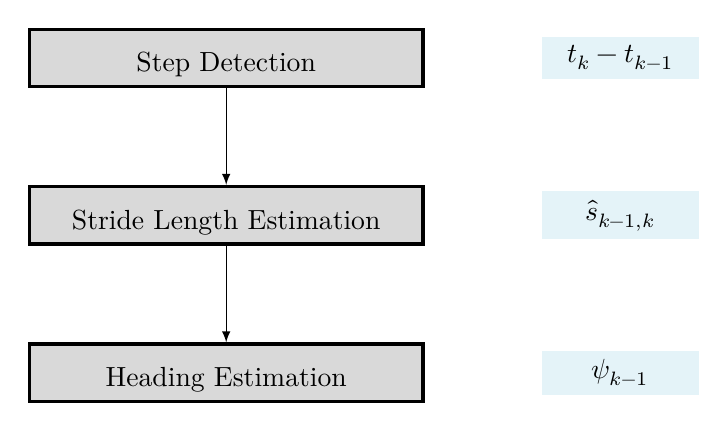
\begin{tikzpicture}
    {[every node/.style={draw, very thick, fill=gray!30, align=center, minimum width=5cm}]
    \node (SD) at (0,0) {步伐探测\\Step Detection};
    \node (SLE) at (0,-2) {步长估计\\Stride Length Estimation};
    \node (HE) at (0,-4) {航向估计\\Heading Estimation};
    }
    {[every node/.style={right=4cm, draw=white, fill=mahiroCloth, minimum width=2cm}]
    \node (SD-text) at (SD) {$t_{k}-t_{k-1}$};
    \node (SLE-text) at (SLE) {$\hat{s}_{k-1,k}$};
    \node (HE-text) at (HE) {$\psi_{k-1}$};
    }
    {[-latex]
      \draw (SD) -- (SLE);
      \draw (SLE) -- (HE);
    }
  \end{tikzpicture}
  \end{figure}
\end{frame}

\subsection{GCJ-02坐标转换}
\begin{frame}
  
  \begin{columns}[c]
    \column{.38\linewidth}
    \begin{figure}[ht]
      \centering
      \includegraphics[width=\columnwidth]{figures/shift.png}
      \caption{\label{fig:shift}卫星影像图和街景图的不重合}
    \end{figure}

    \column{.61\linewidth}
    \setlength{\parskip}{7pt plus 3pt minus 2pt}
    % \begin{itemize}
    % \item 中国GPS偏移问题由GCJ-20和WGS-84基准面不同导致。GPS定位采用的坐标系为WGS-84,投影至以GCJ-02坐标系为基准的街景地图后,会产生非常大(有时超过 \qty{500}{m} )的偏移。
    % \item Google Maps选取GCJ-02坐标系作为街景图的参考系,而卫星影像图仍采用WGS-84,所以会导致如图\ref{fig:shift}偏移问题。
    % \end{itemize}
    中国GPS偏移问题由GCJ-20和WGS-84基准面不同导致。GPS定位采用的坐标系为WGS-84,投影至以GCJ-02坐标系为基准的街景地图后,会产生非常大(有时超过 \qty{500}{m} )的偏移。

    Google Maps选取GCJ-02坐标系作为街景图的参考系,而卫星影像图仍采用WGS-84,所以会导致如图\ref{fig:shift}偏移问题。
  \end{columns}
\end{frame}

\begin{frame}[allowframebreaks]
  经纬度的改正值公式如下:
  \begin{align*}
    \varphi' &=-100+2x+3y+0.2y^2+0.1xy+0.2\sqrt{|x|}\\
    &\ {}+\frac23\left\{[20\sin 6\pi x+20\sin 2\pi x]+\left[20\sin \pi y+40\sin\left(\frac{\pi y}{3}\right)\right]\right.\\
    &\left.\ {}+\left[160\sin\left(\frac{\pi y}{12}\right)+300\sin\left(\frac{\pi y}{30}\right)\right]\right\},\\
    \lambda' &=300+x+2y+0.1(x^2+xy)+0.1\sqrt{|x|}\\
    &\ {}+\frac23\left\{[20\sin 6\pi x+20\sin 2\pi x]+\left[20\sin \pi x+40\sin\left(\frac{\pi x}{3}\right)\right]\right.\\
    &\left.\ {}+\left[150\sin\left(\frac{\pi x}{12}\right)+300\sin\left(\frac{\pi x}{30}\right)\right]\right\}.
  \end{align*}
  其中
  \begin{equation*}
  \begin{cases}
      x=\varphi-105.0,\\
      y=\lambda- 35.0.
  \end{cases}
  \end{equation*}
  之后计算固定值 $(\varphi_\mathrm{fix},\lambda_\mathrm{fix})$:
  \begin{gather*}
  \varphi_\mathrm{fix}=\frac{180\varphi'}{\pi}\cdot\frac{W^3}{a(1-e^2)},\\
  \lambda_\mathrm{fix}=\frac{180\lambda'}{\pi}\cdot\frac{W\cos\left(\mathrm{D2R}(\varphi')\right)}{a},
  \end{gather*}
  式中 $W=\sqrt{1-e^2\sin(\varphi')}$,$a$ 为地球长半径,$e$ 为第一偏心率。
\end{frame}

\section{程序设计流程}
\begin{frame}
  \frametitle{标题}
  测试
\end{frame}

\section{结果展示及精度分析}
\begin{frame}
  测试
\end{frame}

\end{document}